% LaTeX bar chart to compare SAM3 zero-shot runs
% Usage:
% 1) In your document preamble add:
%    \usepackage{pgfplots}
%    \pgfplotsset{compat=1.18}
% 2) Insert this figure environment where needed.

\begin{figure}[htbp]
    \centering
    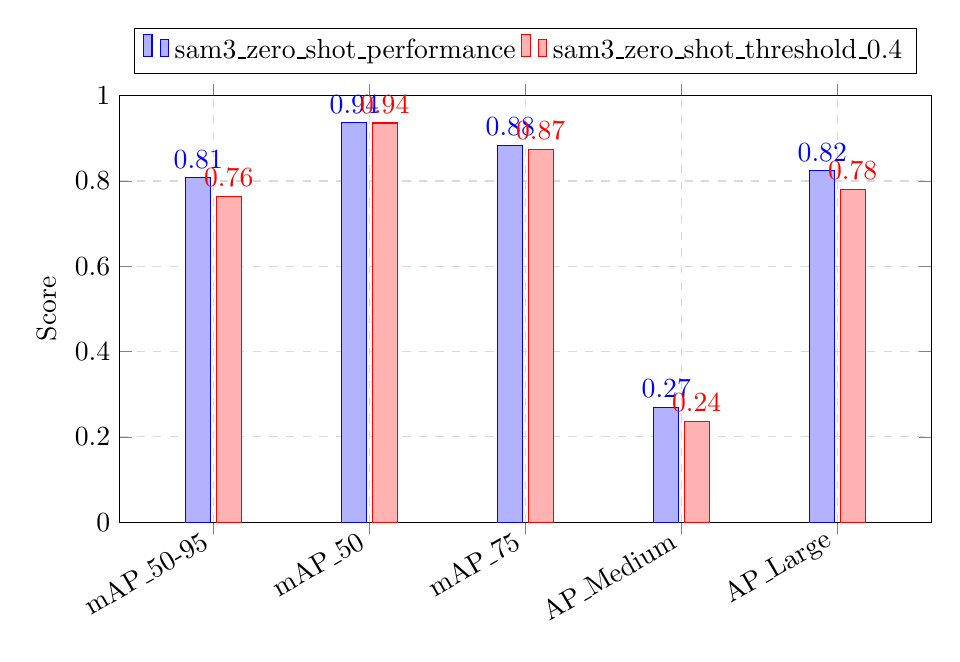
\begin{tikzpicture}
        \begin{axis}[
            ybar,
            bar width=9pt,
            width=0.98\linewidth,
            height=7cm,
            ymin=0,
            ymax=1,
            ylabel={Score},
            symbolic x coords={mAP\_50-95,mAP\_50,mAP\_75,AP\_Medium,AP\_Large},
            xtick=data,
            x tick label style={rotate=30,anchor=east},
            legend style={at={(0.5,1.05)},anchor=south,legend columns=-1},
            nodes near coords,
            nodes near coords align={vertical},
            enlarge x limits=0.15,
            grid=major,
            grid style={dashed,gray!30}
        ]
            \addplot coordinates {
                (mAP\_50-95,0.8074)
                (mAP\_50,0.9361)
                (mAP\_75,0.8838)
                (AP\_Medium,0.2692)
                (AP\_Large,0.8238)
            };
            \addplot coordinates {
                (mAP\_50-95,0.7633)
                (mAP\_50,0.9359)
                (mAP\_75,0.8733)
                (AP\_Medium,0.2357)
                (AP\_Large,0.7806)
            };

            \legend{sam3\_zero\_shot\_performance,sam3\_zero\_shot\_threshold\_0.4}
        \end{axis}
    \end{tikzpicture}
    \caption{Comparison of SAM3 zero-shot metrics from two result files.}
    \label{fig:sam3-zero-shot-comparison}
\end{figure}
